\documentclass[11pt]{article}
\usepackage[margin=1in]{geometry}
\usepackage{graphicx}
\usepackage{multirow}
\usepackage{multicol}
\usepackage{setspace}

\setlength\parindent{0pt}
\usepackage{hyperref}
\usepackage{amssymb,amsthm,amsmath, fancyhdr}
\pagestyle{fancy}

\usepackage{lipsum}

\begin{document}
\chead{Math 121 - Calculating with limit laws}
\begin{enumerate}
\item Justify the use of each limit law used in evaluating the following limit. Write out all steps.
$$\lim_{x \rightarrow 2} \frac{2x^2 + 1}{3x-2}$$
\item Evaluate the following limit, and explain the algebra involved. State what you think would be the most likely mistakes in students evaluating these limits.
\begin{itemize}
\item $$\lim_{h \rightarrow 0} \frac{(-5 + h)^2 - 25}{h}$$

\end{itemize}
\item Find an example of two functions $f$ and $g$, and some real number $a$, such that the limit $\lim_{x \rightarrow a} [f(x) + g(x)]$ exists, but neither $\lim_{x \rightarrow a} f(x)$ or $\lim_{x \rightarrow a} g(x)$ exists.
\item Find an example of two functions $f$ and $g$, and some real number $a$, such that the limit $\lim_{x \rightarrow a} [f(x)g(x)]$ exists, but neither $\lim_{x \rightarrow a} f(x)$ or $\lim_{x \rightarrow a} g(x)$ exists.
\item Suppose that $\lim_{x \rightarrow 1} \frac{f(x) - 8}{x-2} = 10$. Use the limit laws to find $\lim_{x \rightarrow 1} f(x)$.
\item Using the function $f$ illustrated in the following figure, find the following values:
\begin{figure}[h]
\centering
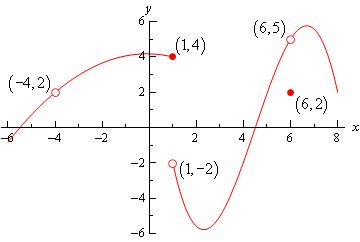
\includegraphics[width=0.8\textwidth]{image004_}
\end{figure}
\begin{itemize}
\item $f(-4)$, $\lim_{x \rightarrow -4^+} f(x)$, $\lim_{x\rightarrow -4^-} f(x)$, $\lim_{x\rightarrow -4} f(x)$
\item $f(1)$, $\lim_{x \rightarrow 1^+} f(x)$, $\lim_{x\rightarrow 1^-} f(x)$, $\lim_{x\rightarrow 1} f(x)$
\item $f(6)$, $\lim_{x \rightarrow 6^+} f(x)$, $\lim_{x\rightarrow 6^-} f(x)$, $\lim_{x\rightarrow 6} f(x)$
\end{itemize}
\item Evaluate the limits as $x$ approaches 2 from both the right and left, and sketch the graph.
$$g(x) = \frac{x^2 + x - 6}{|x-2|}$$
\end{enumerate}
\end{document}